\chapter{Anatomy of spreadsheets and spreadsheet formulas}
\label{chapter:anatomy}

\emph{\small{Parts of this chapter have been published in "A grammar for Spreadsheet Formulas Evaluated on Two Large Datasets" by by Aivaloglou, Hoepelman and Hermans\cite{xlparser}.}}
\vspace{1em}

Altough exotic forms of spreadsheets are available and have been researched, all currently widely used implementation use the following model:
\begin{itemize}
\item A single spreadsheet \key{file} corresponds to a single (\key{work})\key{book}.
\item A workbook can contain any number of (\key{work})\key{sheets}.
\item A sheet consists of a \key{two-dimensional grid} (table) of \key{cells}.
\item A vertical unit in the grid is called a \key{column} and a horizontal unit a \key{row}.
Rows are numbered sequentially top-to-bottom starting at 1, while columns are numbered left-to-right alphabetically, i.e. base-26 using A to Z as digits.
A column or row can also mean all cells contained in that column or row.
\item A \key{cell} can contain a \key{constant value} of any type, a calculation called a \key{formula} or a matrix calculation called an \key{array formula}.
\item An (array) formula can \key{reference} other cells to use their values. When the value of a referenced cell changes, this new value is propagated and the dependent formula values are recalculated.
\end{itemize}

\begin{figure}
\caption{An example dataflow program and its spreadsheet implementation}
\label{fig:dataflow-example}
\centerfloat
\scalebox{0.83}{
\begin{tikzpicture}[-latex ,auto ,node distance =1.3 cm and 1.8cm ,on grid , semithick,
,
state/.style ={ circle ,top color =white ,
draw, minimum width =0.9 cm}]
\node[state] (Input3) {3};
\node[state] (Input5) [below=of Input3] {5};
\node[state] (Plus) [right=of Input5] {$+$};
\node[state] (Input2) [below=of Input5] {2};
\node[state] (Times) [below right=of Plus] {$\times$};
\node[state] (Output) [right=of Times] {\small{\texttt{out}}};
\path (Input3) edge [right] node[right] {} (Plus);
\path (Input5) edge [right] node[right] {} (Plus);
\path (Plus) edge [right] node[right] {} (Times);
\path (Input2) edge [right] node[right] {} (Times);
\path (Times) edge [right] node[right] {} (Output);
%\path (A) edge [loop left] node[left] {$1/4$} (A);
%\path (C) edge [bend left =25] node[below =0.15 cm] {$1/2$} (A);
%\path (A) edge [bend right = -15] node[below =0.15 cm] {$1/2$} (C);
%\path (A) edge [bend left =25] node[above] {$1/4$} (B);
%\path (B) edge [bend left =15] node[below =0.15 cm] {$1/2$} (A);
%\path (C) edge [bend left =15] node[below =0.15 cm] {$1/2$} (B);
%\path (B) edge [bend right = -25] node[below =0.15 cm] {$1/2$} (C);
\end{tikzpicture}
}\hspace{4em}
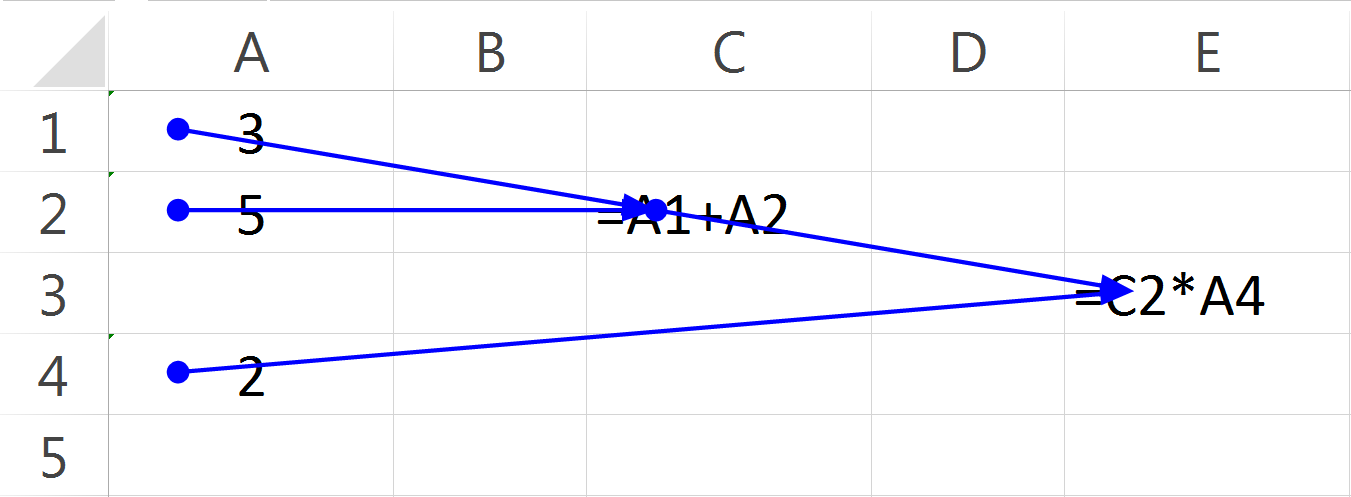
\includegraphics[width=0.5\textwidth]{anatomy/dataflow-program-excel-implementation}
\end{figure}

This model is a variation of the dataflow programming model.
A dataflow program is a directed graph, where data flows between operation in nodes along the graphs edges.
In spreadsheets, cells represent the nodes of a dataflow program and edges are represented by references.
An example dataflow program and its spreadsheet implementation can be seen in Figure \ref{fig:dataflow-example}.

The spreadsheet model is Turing complete, as proven by an Excel 2010 implementation of a Turing machine \cite{ExcelTuringComplete}.

\section{Formulas}

Formulas consist of expressions which can contain constant values, \key{function calls} and \key{operators} and, most importantly, \key{references} to other cells.
A cell is identified as a formula cell because all formulas must start with the equals sign \f{=}.

\subsection{Function calls and operators}

Function calls are done by starting with the function name, followed by the arguments in parentheses, separated by a comma.
All spreadsheet implementations provide a range of built-in functions, and in most spreadsheet implementations it is possible to define new functions yourself.
However this is not done directly inside the spreadsheet, and uses an alternate programming language.
In Microsoft Excel and Openoffice.org/Libreoffice this is done with a variant of the BASIC programming language, while in Google Docs this is done with Javascript.

The operators \f{+ - * / = <> <= < >} and \f{>=} can be used according to their usual semantics.
\f{+} and \f{-} are available both unary (\f{=-1}) and binary (\f{=1-1}).
Additionally the \f{\%} unary operator is defined to transform a number into a percentage, \f{\^} is the exponentiation operator and \f{\&} is the text concatenation operator.

Spreadsheets contain three fairly unique binary operators with the range operator \f{:}, the union operator \f{,} and the intersection operator \f{\char32}.
Te semantics of these operators are detailed in section \ref{sec:references}.

\subsection{References}
\label{sec:references}
References are the core component of spreadsheets.
The value of any cell can be used in a formula by concatenating its column and row number, producing a reference like \f{B5}.
This is called A1-style referencing and is by far the most comment in modern spreadsheet implementations.
If the value of a cell changes this new value will be propagated to all formulas that use it.

When copying a cell to another cell by default references will be adjusted by the offset, for example copying \f{=A1} from cell B1 to C2 will cause the copied formula to become \f{=B2}.
This can be prevented by making the reference absolute by prepending a \f{\$} to the column index, row index or both.
The formula \f{=\$A\$1} will remain the same on copy while \f{=\$A1} will still have its row number adjusted when copied.

\subsection{Ranges}
References can also be \emph{ranges}, which are collections of cells.
Ranges can be constructed by three operators: the range operator \f{:}, the union operator \f{,} (a comma) and the intersection operator \f{\char32} (a space).
The range operator \f{:} creates a rectangular range with the two cells as top-left and bottom-right corners, so \f{=SUM(A1:B10)} will sum all cells in columns A and B with row number 1 through 10.
The range operator is also used to construct ranges of whole rows or columns, for example \f{3:5} is the range of the complete rows three through five, and \f{A:D} is the range of columns A through D.
The union operator, which is different from the mathematical union as duplicates are allowed, combines two references, so \f{A1,C5} will be a range of two cells, \f{A1} and \f{C5}.
Lastly the intersection operator takes only the cells which are in both arguments, \f{=A:A 5:5} will thus be equivalent to \f{=A5}.

A user can also give a name to any collection of cells, thus creating a \emph{named range} which can be referenced in formulas by name.

\subsection{Structured References}

A recent addition to the formula language introduced in Excel 2007 are structured (table) references.
To use this feature, a table can be given a name and must have headers.
One can then reference a column in the table by entering \f{TableName[ColumnName]}.
Inside the square brackets reference operators can be used to construct more complex references, \f{TableName[Column1,Column4]} references two columns.
Several keywords 

There is no way to reference a specific row, except the current row, for example if a formula is places in \f{A3} it can only reference row number 3.
The \f{\#This Row} keyword and the \f{@} operator are used for this: \f{TableName[\#This Row]} and \f{TableName[@]} both reference the current row number in the provided table, and \f{TableName[@ColumnName]} references the cell in the provided column of the current row number.

This feature is meant to make formulas easier to read, by references in a formula like \f{=SUM(F1:F10)-SUM(I1:I10)} with human-readable names like \f{=SUM(Budget[Revenue]) - SUM(Budget[Expenses])}.

\subsection{R1C1 reference style}

An alternate style called R1C1 as opposed to the above A1 style exists, but it is very rarely seen or used by users.
In R1C1 reference style one specifies either the offset to a cell between square brackets or its concrete location.
In R1C1 style \f{R[4]C[-2]} means the cell two columns to the left and four rows down, while \f{R2C2} refers to cell B2.
The biggest advantage of R1C1 is that it causes identical formulas to be the same even when they operate on different cells or data because of their position.
These properties make R1C1 useful as an internal representation in spreadsheet implementations.

\subsection{Inter-sheet and external references}
\label{subsection:ExternalRefsDDE}

By default references are to cells or ranges in the same sheet as the formula, but this can be modified with a prefix. A prefix consists of some identifier, followed by an exclamation mark followed by the actual reference.

The most common use case is to reference another sheet in the same workbook, where the prefix is simply the sheet name: \f{=Sheetname!A1}.
References to external spreadsheet files are also possible, which is done by prepending the file name in between square brackets: \f{=[Filename]Sheetname!A1} or \f{=[Filename]!NamedRange}.
A peculiar type of prefix are those that indicate multiple sheets: \f{=Sheet1:Sheet10!A1} means A1 in Sheet1 through Sheet10.
Sheet names can also be between single quotes: \f{='Sheetname with space'!A1}. 

In Windows versions of Microsoft Excel formulas can also call external programs through Dynamic Data Exchange (DDE).
DDE links are a special case of references, used for receiving data from other applications.
They take the form of \f{=Program|Topic!Arguments}, e.g. \f{=Database|TableA!Column1}.

\subsection{Case sensitivity}

Formulas are case-insensitive outside string literals.
Identifiers have a canonical capitalization, and while user can type the identifier with any casing only the canonical form will be displayed.
While the canonical capitalization of built-in identifiers,functions and reserved names, is usually uppercase, the canonical capitalization of an user-defined identifier, an user defined function or a named range, is as the user defined it originally.

\subsection{Whitespace sensitivity}

The excel formula language is whitespace sensitive in several places:
\begin{itemize}
\item Inside string literals
\item To separate syntactic units: \f{=AB} has a different meaning than \f{=A B}
\item Whitespace is not allowed between function names and the argument list: \f{=SUM  (1)} is invalid.
\item Whitespace is not allowed inside internal or external references: \f{=Sheet1 !A1} is invalid.
\item The intersection operator is a single space: \f{=A:A 3:3} is the intersection of column \f{A} and row \f{3}, equivalent to \f{=A3}
\end{itemize}

\section{Array Formulas and Arrays}
\label{sec:arrayformulas}
In spreadsheet programs it is possible to work with one- or two-dimensional matrices.

When constructed from constant values they are called \emph{array constants}, e.g. \f{\{1,2;3,4\}}.
They are surrounded by curly brackets, columns are separated by commas, and rows by semicolons.
Several matrix operations are available, for example \f{=SUM(\{1,2,3\}*10)} will evaluate to 60.

\emph{Array Formulas} use the same syntax as normal formulas, except that the user must enter \emph{Ctrl} + \emph{Shift} + \emph{Enter} to signal that it is an Array formula.
Excel and LibreOffice surround the formula with curly braces.
Google docs works differently and requires the user to surround an array formula with \f{ARRAYFORMULA($\ldots$)}.

Marking a formula as an array formula will enable one- or two-dimensional reference ranges to be treated as matrices, and several matrix operators and functions will be available and allow a formula to return multiple values, to be displayed in multiple cells.
For example if \f{A1},\f{A3},\f{A3} contain the values \f{1},\f{2},\f{3} the array formula \f{\{=SUM(A1:A3*10)\}} will evaluate to \f{60}.
Furthermore, an array formula allows the user to return multiple results, which will be presented in multiple cells.
The array formula \f{\{=\{1,2,3\}*\{4,5,6\}\}} will show \f{4}, \f{10} and \f{18} in three different cells.

\section{Type system}

The type system in Microsoft Excel is weak with most typed being able to be coerced into others.
Explicit type conversion is done by certain built-in functions.
For values inside formulas, the following types exist:

\begin{itemize}
\item[Boolean] values are either \f{TRUE} or \f{FALSE}. Booleans can be coerced to numbers where \f{TRUE} will become 1 and \f{FALSE} will become 0 and strings.
\item[Numeric] values are in the range of 8-byte IEEE doubles. Numbers can be provided as integers, decimals or in scientific notation.
When coerced to booleans 0 will become \f{FALSE}, all other values will be \f{TRUE}. Number can also be coerced into strings.
\item[String] values are any Unicode character enclosed in quotation marks \f{"}.
Two quotation marks serve as the escape character, thus \f{""""} represent the string ".
If the contents of a cell start with a \texttt{'} the rest of that cell content is interpreted as a string.

When coerced to booleans all strings except the empty string are \f{TRUE}, the empty string is \f{FALSE}.
When coerced to a numeric value the spreadsheet program will accept any string representing valid numeric user input and otherwise give the error \f{\#VALUE!}.
\item[Error] values are \f{\#DIV/0!}, \f{\#NAME?}, \f{\#NULL!}, \f{\#NUM!}, \f{\#N/A!}, \f{\#VALUE!} and \f{\#REF!}.
Errors behave similar to exceptions or the maybe monad in that they will propagate throughout a calculation.

Errors cannot be coerced, but can be explicitly converted by functions such as \f{ISERROR}.

\item[Ranges and arrays] are one- or two-dimensional matrices of any non-array values. Arrays are rarely used outside of array formulas, but ranges are very common in formulas.
However, these types usually only serve as inputs for functions and are thus fairly transparent to the user outside of array formulas.
Both types usually cannot generally be, doing so will result in the \f{\#VALUE!} error.
\end{itemize}

Some other "display types" exists, these can change the way the data is presented to or validated from the user and can have implications when inter-operating with other programs.
Usually the user can mark a cell as containing one of these types, or Excel can automatically mark a cell to be of this type based on heuristics.
In formulas and internally these types are all represented by one of the above types.
A few of these are commonly used:
\begin{itemize}
\item[Dates and times] are internally stored as a floating point with the integer portion being the number of days since an the epoch January 1st 1900, incorrectly considering 1900 a leap year, and the remainder being the portion of the day that passed.
Excel displays dates and times as is customary in the locale of the user.
When interoperating a date or time value will be exported as a datetime type value of that system.
\item[Currency] is stored as other numbers and displayed in the format customary for the specific currency. When interoperating with some other systems currency values will be exported using arbitrary-precision arithmetic formats.
\item[Percentages] are stored as other numbers, but displayed as if multiplied by 100\%.
\end{itemize}